% Building and training deformable models of objects (e.g. faces, ears, bodies, bottles, vehicles etc.) has recently been widely researched for object detection, part localisation, fitting, recognition and tracking using manual annotated data. Shapes and appearances of majority of objects vary significantly from object instance. To illustrate, ears have complicated inner structures (e.g. helix, crus antihelicis, scapha, tragus, lobe etc.) which differs remarkably between ears and highly sensitive to intensity changes. Recently, we have witnessed a great progress in object detection, alignment and recognition.

% To train deformable models with satisfiable generalisation, large amount of careful manual annotation is required. However, landmark annotation is extremely time consuming, work intensive and, most importantly, number of landmarks have to stay consistent for all training data while it is challenging to maintain the consistency or to avoid bias when annotating objects that having reach features. In ears, for example, large amount of landmarks required as the inner structure of ears are complex. To annotate an ear with clear contour, helix and cavum conchae, more than 50 landmarks are required. The inconsistency of ear features enhanced the difficulty of accurate annotation (e.g. Fossa Triangularies and Crus Helicis are optional feature of an ear also their visibility is highly sensitive to pose and illumination variation).
% To illustrate how much time consuming careful ear annotation is, according to our experience, a trained annotator may need an average of (TODO: experiment) minutes per image for the manual annotation of 55 landmarks. This means that the annotation of 1000 images requires a total of about (TODO: experiment). Furthermore, personal issue, prior knowledge and circumstances can heavily bias the annotation accuracy thus second round correction might desired.

% We propose a framework to (1) construct SDMs using training data with inconsistent annotation, (2) introduce highly effective curve annotation which tremendously reduces manual work overload but maintains same performance level against state-of-the-art SDMs and (3) build dense correspondent SDMs with shape flow.

% %(1)
% Annotated data of same objects can have various number of landmarks, \cite{?} shown faces have landmarks different in range 10+ to 70+. Building SDMs (e.g. Active Appearance Models), however, require training data are annotated consistently, for example, all faces have 68 landmarks, 6 landmarks for an eye and 9 for a nose \cite{?}. Such property of SDMs largely limited their application area like combining different dataset as one. We propose the pipeline with non-rigid alignment and support vector shape to blend landmarks into relatively consistent shape discriminator before building models.

% %(2)
% Due to the fact that manual annotation is a rather costly and labour-intensive procedure, unsupervised and semi supervised learning of models for the tasks of alignment, landmark localisation, tracking and recognition has attracted considerable attention \cite{?}. As our proposed framework are available to handle landmarks with inconsistency, it leads to a more efficient, convenient, unbiased and simple annotation methods - curve annotation.

% %(3)
% To build dense correspondence between independent shapes, we apply optical flow on shapes with low rank constrains, so we name it shape flow. Optical flow is originally applied to video sequences that several assumptions holds, illumination consistency and motion smoothness, while shapes having no motion smoothness completely as all training data are independent. Low rank constrain plays important role to simulate motion smoothness assumption.


% % Back Ground, uses Nondas' paper "Automatic Construction of Deformable Models In-The-Wild" as place holder
% The two most closely related works to the proposed
% method are the automatic construction of Active Appearance
% Models (AAMs) in \cite{?} and the so-called RASL
% methodology in \cite{?} for person-specific face alignment.
% There are two main differences between our framework
% and \cite{?}. (1) We use a predefined statistical shape model
% instead of trying to find both the shape and appearance models.
% We believe that with the current available optimization
% techniques, it is extremely difficult to simultaneously optimize
% for both the texture and shape parameters. (2) We
% employ the robust component analysis of \cite{?} for the appearance
% which deals with outliers. Thus, even though
% our method is similar in concept to \cite{?}, these two differences
% make the problem feasible to solve. In particular, the
% methodology in \cite{?} fails to create a generic model even in
% controlled recording conditions, due to extremely high dimensionality
% of the parameters to be found and to the sensitivity
% of the subspace method to outliers. This was probably
% one of the reasons why the authors demonstrate very
% limited and only person-specific experiments. Furthermore,
% our methodology bypasses some of the limitations of \cite{?},
% which requires the presence of only one low-rank subspace,
% hence it has been shown to work only for the case of congealing
% images of a single person. Finally, we argue that
% in order for an automatically constructed AAM methodology
% to be robust to both within-class and out-of-class outliers4,
% which cannot be avoided in totally unsupervised setting
% statistical component analysis techniques should be
% employed \cite{?}.

% We summarize our contributions as follows:
% \begin{itemize}
%   \item Constructing SDMs using training data with inconsistent annotation.
%   \item Introduce highly effective curve annotation which tremendously reduces manual work overload but maintains same performance level against state-of-the-art SDMs.
%   \item Building dense correspondent SDMs with shape flow
% \end{itemize}

% In our experiment, we show that building robust dense models trained with inconsistent annotation and trained with curve annotation improves performance of discriminative models trained on carefully annotated data including ears, faces, bottles, (cars ?) and bodies. Evaluation methods and choices are described in details.


% \clearpage

\begin{figure}[t!]
    \centering
    \begin{subfigure}[b]{0.105\textwidth}
            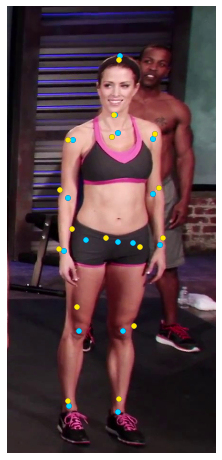
\includegraphics[height=5.5cm]{resources/MotivativeAnnotation/MPII}
            \caption{MPII}
    \end{subfigure}
    \hfill
    \begin{subfigure}[b]{0.115\textwidth}
            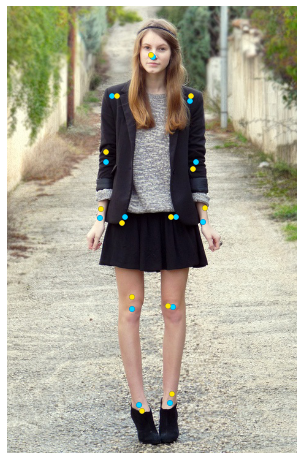
\includegraphics[height=5.5cm]{resources/MotivativeAnnotation/FashionPose}
            \caption{Fashion}
    \end{subfigure}
  	\hfill
    \begin{subfigure}[b]{0.22\textwidth}
            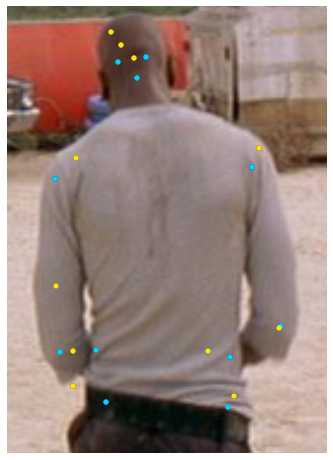
\includegraphics[height=5.5cm]{resources/MotivativeAnnotation/FLIC}
            \caption{FLIC}
    \end{subfigure}
    % \hfill
    % \begin{subfigure}[b]{0.145\textwidth}
    %         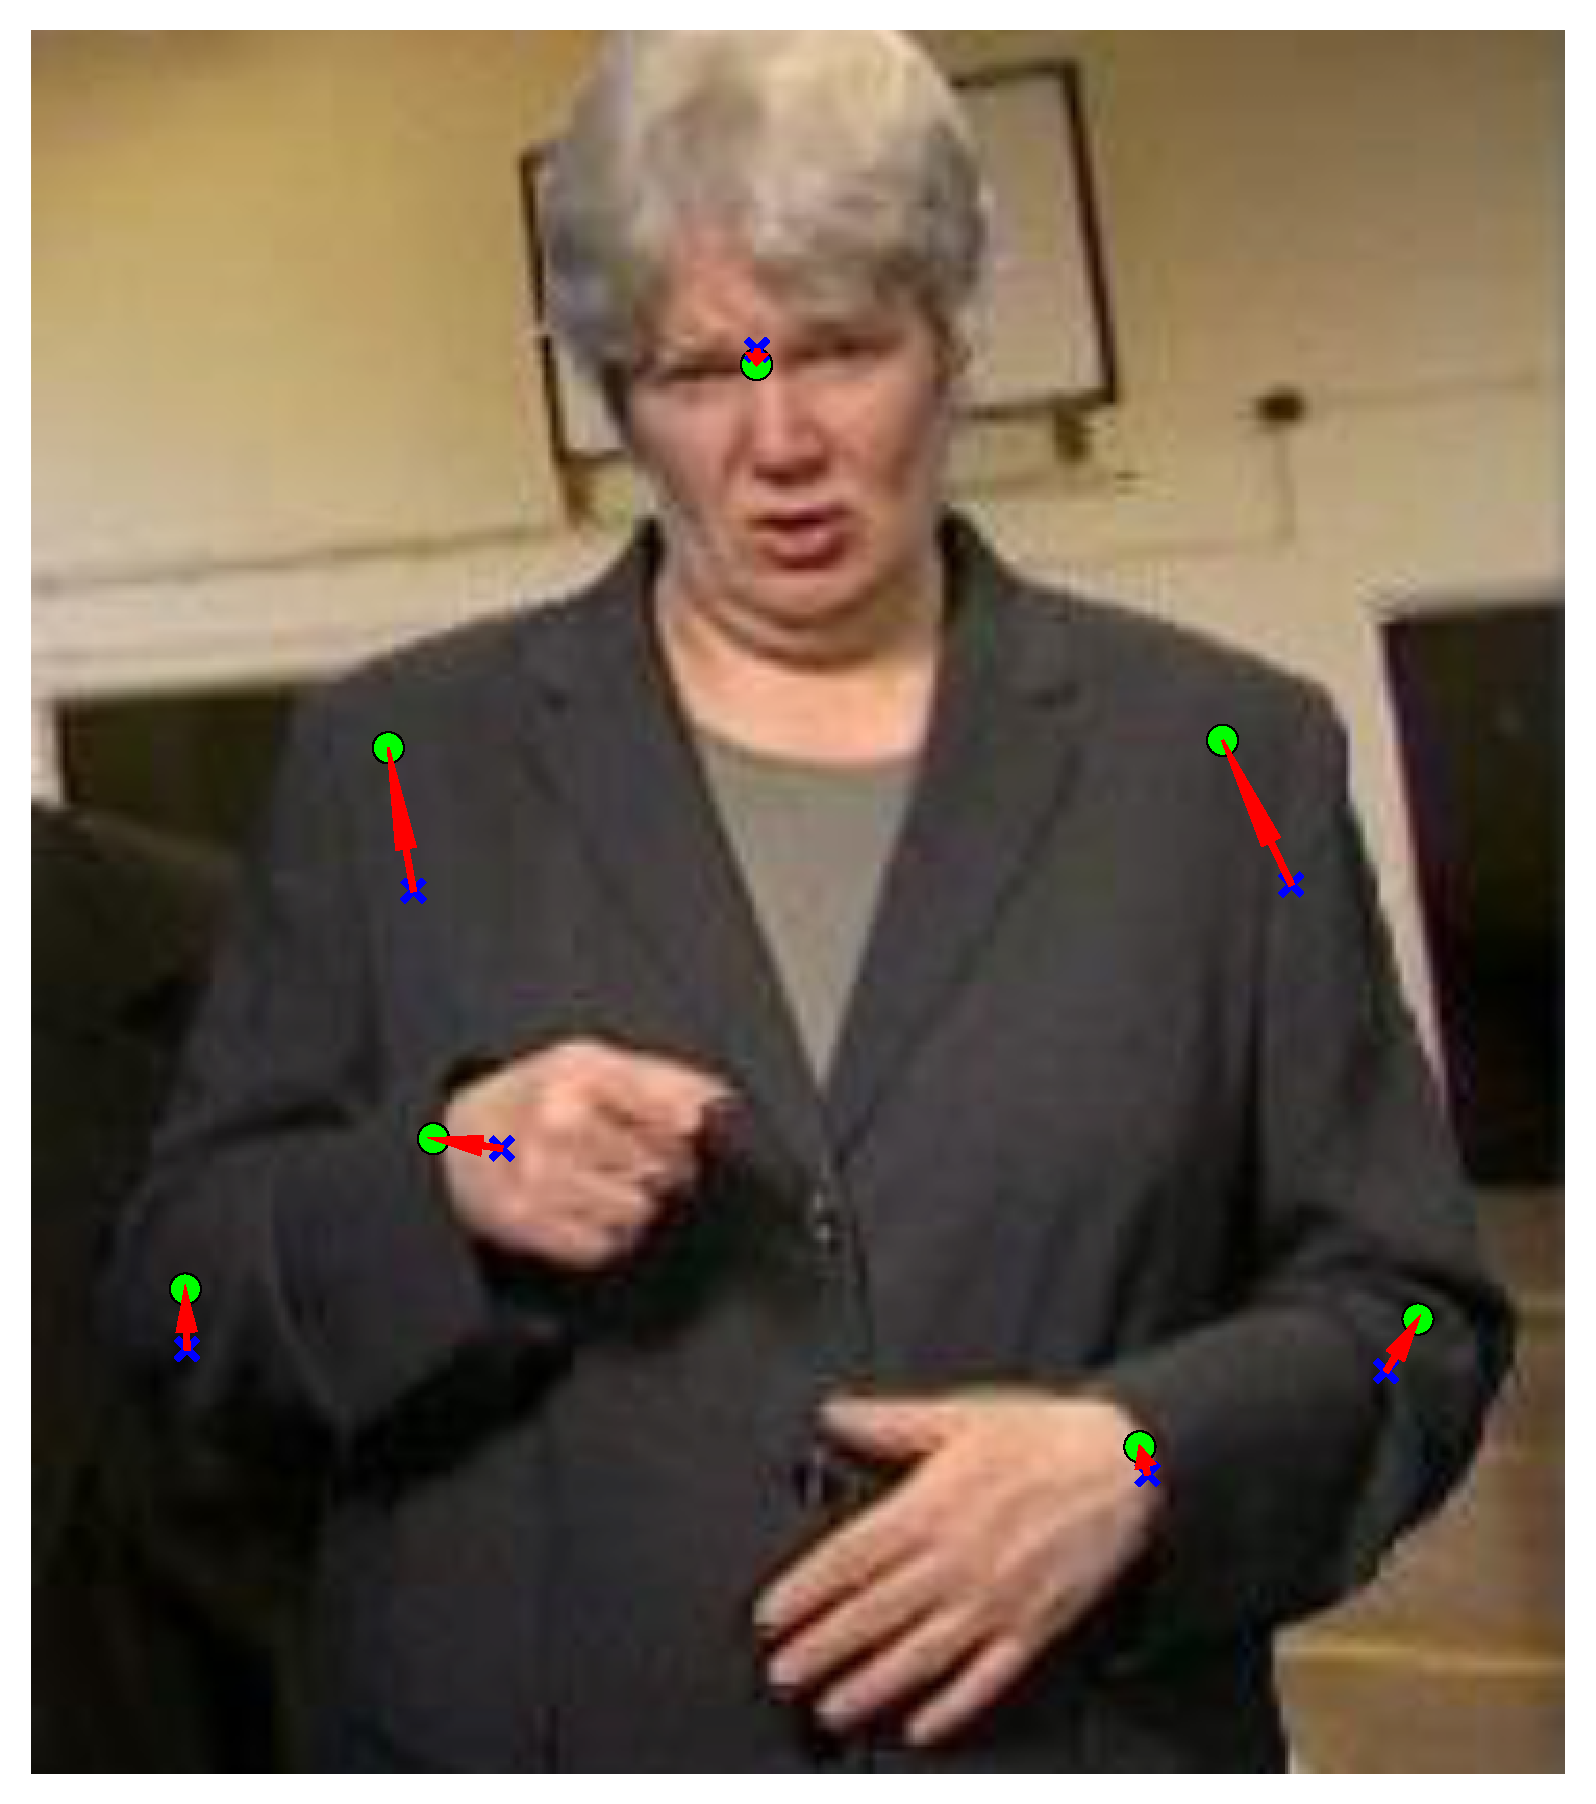
\includegraphics[height=4cm]{resources/MotivativeAnnotation/BBCPose}
    %         \caption{BBC Pose}
    % \end{subfigure}
    \caption{Examples of inconsistent and inaccurate annotations of human pose among different datasets. \emph{Blue} dots denote the original annotations. The arrows and \emph{green} dots show the correct location at which the points should be.
    %Original annotations are shown in blue dots while better annotations shown in green dots.
    }
    \label{fig:wrong_anno}
\end{figure}
\begin{figure}[t!]
    \centering
    \begin{subfigure}[b]{0.065\textwidth}
            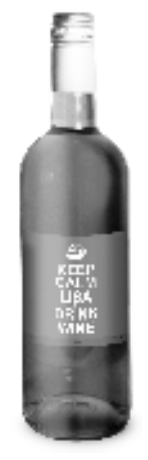
\includegraphics[height=2.55cm]{resources/Fig_Intro/intro_2_0}
    \end{subfigure}
    \hfill
    \begin{subfigure}[b]{0.065\textwidth}
            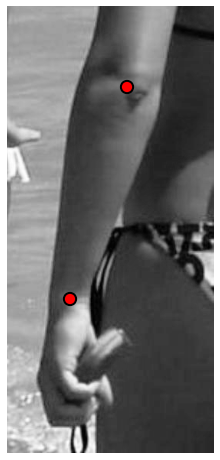
\includegraphics[height=2.55cm]{resources/Fig_Intro/intro_2_1}
    \end{subfigure}
    \hfill
    \begin{subfigure}[b]{0.065\textwidth}
            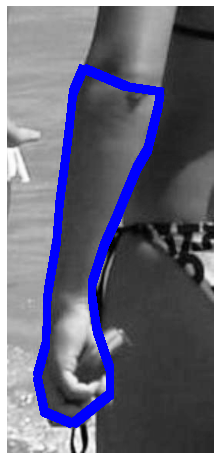
\includegraphics[height=2.55cm]{resources/Fig_Intro/intro_2_2}
    \end{subfigure}
    \hfill
    \begin{subfigure}[b]{0.085\textwidth}
            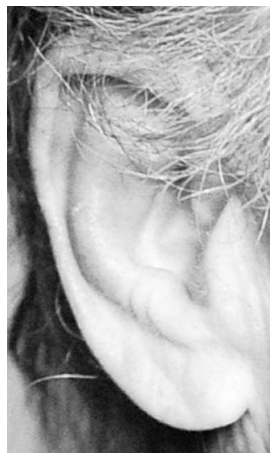
\includegraphics[height=2.55cm]{resources/Fig_Intro/intro_1_0}
    \end{subfigure}
    \hfill
    \begin{subfigure}[b]{0.085\textwidth}
            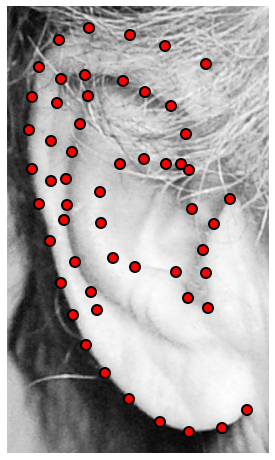
\includegraphics[height=2.55cm]{resources/Fig_Intro/intro_1_1}
    \end{subfigure}
    \hfill
    \begin{subfigure}[b]{0.085\textwidth}
            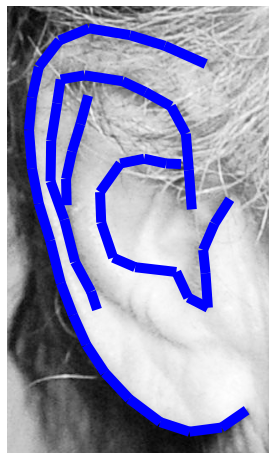
\includegraphics[height=2.55cm]{resources/Fig_Intro/intro_1_2}
    \end{subfigure}
    \\
    \begin{subfigure}[b]{0.156\textwidth}
            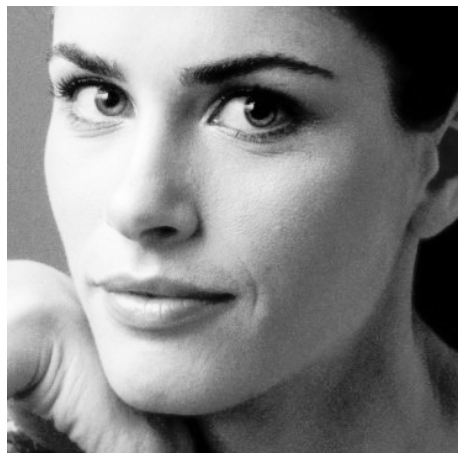
\includegraphics[height=2.8cm]{resources/Fig_Intro/intro_0_0}
    \end{subfigure}
    \hfill
    \begin{subfigure}[b]{0.156\textwidth}
            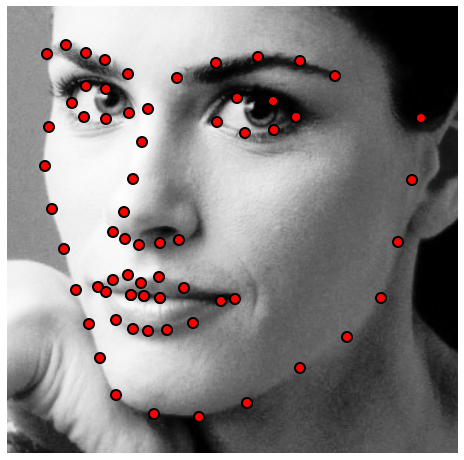
\includegraphics[height=2.8cm]{resources/Fig_Intro/intro_0_1}
    \end{subfigure}
  	\hfill
    \begin{subfigure}[b]{0.156\textwidth}
            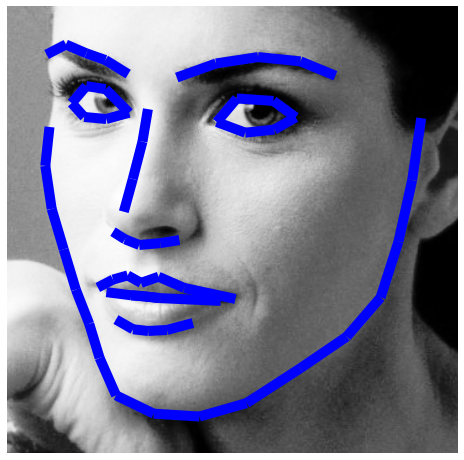
\includegraphics[height=2.8cm]{resources/Fig_Intro/intro_0_2}
    \end{subfigure}
    \caption{Comparison of the standard landmark annotation (\emph{red} dots) with the curve annotation (\emph{blue} lines) on arms, ears and faces. It is evident that the curve annotations surpass the inevitable inconsistency of sparse annotations.}
    \label{fig:intro}
\end{figure}


Statistical Deformable Models (SDMs) of various object classes is a well-studied and popular area in the intersection of computer vision and machine learning \cite{Cootes1995, Cootes2001, Matthews2004, Saragih2011, Belhumeur2011, Zhu2012, Xiong2013}. Recently, we have witnessed tremendous developments on SDMs of human faces and bodies trained with images that are captured under unconstrained conditions, usually referred to as ``in-the-wild" \cite{Belhumeur2011, Cao2012, Zhu2012, Xiong2013, Asthana2013, Tzimiropoulos2014, Asthana2014}. This is attributed to:
\begin{itemize}
\item The abundance of complex visual data, spread through web services (e.g. Youtube, Flickr, Google Images), which has led to the development of ``in-the-wild" databases of human faces and bodies \cite{Belhumeur2011, Le2012, Zhu2012, Burgos2013}.

\item The manual annotation of such databases that has been undertaken by several research teams \cite{sagonas_iccv_300w_2013,charles2013domain,dantone2014body,andriluka14cvpr}.

\item The development of powerful visual features that are able to describe objects and their parts in a robust manner (e.g., SIFT \cite{lowe1999object}, HoGs \cite{Dalal2005}
%and Deep Convolutional Neural Networks \cite{sermanet2013overfeat}
), as well as generative and discriminative methodologies for learning SDMs.
\end{itemize}

However, there are two main drawbacks when building SDMs directly on manually annotated landmarks:
\begin{itemize}

\item Annotating with regards to consistent landmarks is an extremely time consuming, tedious and labour intensive work \cite{sagonas_iccv_300w_2013}, which is usually performed by a trained person. Furthermore, for various object classes, it requires a highly skilled person in order to identify and annotate landmarks in a consistent manner. For example, the human ear has very complicated inner structures (helix, crus antihelicis, scapha, tragus, lobe etc.) which remarkably differ between different ears. Moreover, certain ear parts, such as fossa triangularies and crus helicis, do not appear in all ears and their visibility is highly sensitive to the head pose and illumination variation. Another such example is the human body, which is generally annotated with regards to a number of landmarks that intuitively correspond to a set of body joints. For most body pose databases, annotation task was undertaken by a crowd-sourcing Internet marketplace, so-called Amazon Mechanical Turk (AMT). Unfortunately, this resulted in acquiring inconsistent and inaccurate annotations, in many cases\footnote{In the case of faces, the quality of annotations produced from AMT are extremely inaccurate and cannot, by any means, be compared with the ones provided by the recent 300W competition \cite{sagonas_iccv_300w_2013}.} (please see Figure \ref{fig:wrong_anno}). As it was also recently pointed out \cite{tompson2015efficient}, the inconsistencies in body joint annotations may also render the comparison between different human pose estimation methodologies irrelevant.

\item The nature of many deformable objects does not allow them to be annotated with regards to a consistent set of landmarks (e.g., bottles, fruits etc.). Additionally, it is very difficult to consistently annotate the boundary/outline of certain objects such as faces, ears, body, since these landmarks do not have any semantic meaning. That is why many state-of-the-art methods opt to leave the boundary out when reporting results \cite{Tzimiropoulos2014, Asthana2014}. The majority of the state-of-the-art methods for model-based landmark localisation \cite{Cao2012, Zhu2012, Xiong2013, Tzimiropoulos2014, Asthana2014} are not applicable to objects with inconsistent sets of landmarks.

\end{itemize}

To illustrate how time consuming careful annotation of a complex deformable object is, we lay down our own experience based on the human ear. A trained annotator needs an average of 4 minutes per image for the manual annotation of 55 landmarks. This means that the annotation of 1000 images requires a total of about 67 hours. Furthermore, the quality of training as well as fatigue largely influence the annotation accuracy. Hence, a second pass on the annotated data is, in many cases, necessary. Due to the fact that manual annotation is a costly and labour-intensive procedure, unsupervised learning of deformable models for the task of object alignment has recently attracted some attention \cite{frey2003learning, baker2004automatic, cootes2004groupwise, jojic2006escaping, Huang2006, kokkinos2007unsupervised, jiang2009learning, liu2009simultaneous, Zhang2012}. However, because the problem of fully unsupervised discovery of the deformations of arbitrary objects is difficult and ill-posed, the limited number of methods that have been proposed for the task cannot be directly applied to arbitrary collection of ``in-the-wild" images. On the other hand, the method of \cite{antonakos2014automatic}, which can deal with ``in-the-wild" images, requires a set of consistently annotated sparse shapes to perform deformable face congealing.


\section{Contributions}

In this paper, we propose a solution for annotating an object with regards to its deformations that requires considerably less effort compared to manual annotation and, at the same time, can be used to define statistical deformations for objects without a consistent set of landmarks. We employ the proposed method in order to construct SDMs based on the outline of human body parts (i.e., arms and legs). To the best of our knowledge, this is the first time that an SDM is proposed to be trained on the outline of human body parts and not on their skeleton joints. The proposed SDM can also be used to provide accurate and consistent annotations for several of the body joints (such as wrist, elbow etc.).

To this end, we argue and empirically demonstrate that it is better to annotate an object with regards to a set of continuous lines that describe its shape. An example is provided in Figure \ref{fig:intro}, which compares the standard landmark annotations that are employed in the current literature with the proposed curve annotations for arms, ears and faces. It becomes evident that the curve annotations avoid the inherent ambiguity of placing sparse landmarks and offer a richer description of the object's shape.
%
%where the shape of the human arm is annotated with continuous lines instead of a number of discrete landmarks. Similarly, the shape annotations for an ear and a face are shown in the same figure. Annotating images by following this procedure takes 42, 38 and 43 secs per image for arm, faces, ears correspondingly.
Furthermore, these curves can be automatically generated by recently proposed methods that perform discriminative segmentation of objects \cite{luo2013pedestrian,liu2015matching}.

Furthermore, we capitalise on recent advances on multiframe optical flow estimation \cite{Garg:2013hu} and show that the relevant methodologies have matured enough to densely annotate the proposed shapes using either simplistic or even more sophisticated and robust shape representation methods \cite{Nguyen2013}.
In particular, in order to build dense correspondences between different shape instances of the same object class, we jointly estimate the optical flow among all the instances by imposing low-rank constrains, an approach that we call \emph{Shape Flow}. Multiframe optical flow has originally been applied on video sequences, relying on the assumptions of color consistency and motion smoothness \cite{Garg:2013hu}. However, these assumptions do not hold in our case, where we have a collection of shapes. Therefore, we introduce appropriate modifications based on the consistency of image-based shape representation, as well as low rank priors.
%
%On the other hand,  while shapes having no motion smoothness completely as all training data are independent. Low rank constrain plays important role to simulate motion smoothness assumption.

In addition, we demonstrate how dense Active Appearance Models (AAMs) can be built after establishing dense shape correspondences. We show that the proposed methodology can be applied on landmark localisation, even though it is not tailored for that task, achieving particularly good performance. We also illustrate the performance of the proposed methodology for describing objects that do not have consistent landmarks. Furthermore, we show how to build a powerful part-based AAM on the sparse outline landmarks that are obtained by sampling the shape of the dense AAM. Using the resulting outline part-based AAM, we report state-of-the-art performance on the task of human body parts localisation on challenging databases. Finally, we show that the proposed part-based AAM can be used to provide consistent annotations for different body parts.


%To the best of our knowledge this is the first methodology which can %create a dense statistical model for AAM which can operate in %"in-the-wild".

%[..]. There are methods such as [..] and [..] but ...

In summary, the contributions of this paper are the following:
\begin{itemize}

  \item We propose one of the first methodologies that build accurate SDMs from a set of training data with inconsistent annotations. We show that the proposed methodology, thanks to the highly effective curve annotations, tremendously reduces manual workload but maintains same performance level against state-of-the-art SDMs. We show that by sampling the dense shape of SDM very powerful part-based SDMs can

  \item We propose the first SDMs of the outline of human parts, such as human arms, which can be applied for both highly accurate body part segmentation and pose estimation, as well as for providing accurate annotations for body joints.

\end{itemize}



%In our experiment, we show that building robust dense models trained with inconsistent annotation and %trained with curve annotation improves performance of discriminative models trained on carefully %annotated data including ears, faces, bottles, (cars ?) and bodies. Evaluation methods and choices are %described in details.




%We propose a framework to (1) construct SDMs using training data with inconsistent annotation, (2) %introduce highly effective curve annotation which tremendously reduces manual work overload but %maintains same performance level against state-of-the-art SDMs and (3) build dense correspondent SDMs %with shape flow.

%(1)
%Annotated data of same objects can have various number of landmarks, \cite{?} shown faces have %landmarks different in range 10+ to 70+. Building SDMs (e.g. Active Appearance Models), however, %%require training data are annotated consistently, for example, all faces have 68 landmarks, 6 landmarks %for an eye and 9 for a nose \cite{?}. Such property of SDMs largely limited their application area like %combining different dataset as one. We propose the pipeline with non-rigid alignment and support vector %shape to blend landmarks into relatively consistent shape discriminator before building models.

%(2)



%(3)


% Back Ground, uses Nondas' paper "Automatic Construction of Deformable Models In-The-Wild" as place holder
%The two most closely related works to the proposed
%method are the automatic construction of Active Appearance
%Models (AAMs) in \cite{?} and the so-called RASL
%methodology in \cite{?} for person-specific face alignment.
%There are two main differences between our framework
%and \cite{?}. (1) We use a predefined statistical shape model
%instead of trying to find both the shape and appearance models.
%We believe that with the current available optimization
%techniques, it is extremely difficult to simultaneously optimize
%for both the texture and shape parameters. (2) We
%employ the robust component analysis of \cite{?} for the appearance
%which deals with outliers. Thus, even though
%our method is similar in concept to \cite{?}, these two differences
%make the problem feasible to solve. In particular, the
%methodology in \cite{?} fails to create a generic model even in
%controlled recording conditions, due to extremely high dimensionality
%of the parameters to be found and to the sensitivity
%of the subspace method to outliers. This was probably
%one of the reasons why the authors demonstrate very
%limited and only person-specific experiments. Furthermore,
%our methodology bypasses some of the limitations of \cite{?},
%which requires the presence of only one low-rank subspace,
%hence it has been shown to work only for the case of congealing
%images of a single person. Finally, we argue that
%in order for an automatically constructed AAM methodology
%to be robust to both within-class and out-of-class outliers4,
%which cannot be avoided in totally unsupervised setting
%statistical component analysis techniques should be
%employed \cite{?}.

